
\begin{itemize}
	\item Initial ideas around technical challenges
	%(Possibly any initial ideas you have around solving some of the technical challenges)
	\begin{itemize}
		\item[] To start off, we would implement a server that would be hosted in a cloud. The server will be accessed via the presenters' or the meeting leaders' computer. It will then comunicate with a gateway device (Intel Edison) which in turn will communicate with the node(s). Each node will be equiped with a NFC writer/reader to enable us to log the person into the meeting and send the agenda to his/her phone. We decided that there should be the possibility for more than one person to tap in at a time. When a user taps in, his/her screen would notify them when the phone is safe and when it is restored.
		\item[] The malware is a tricky part of this project, but we think we would be able to get root or super user access to the phones' OS through creative techniques. Thus enabling us to use the victims phone as we wish.
	\end{itemize}
	
	\item Progress Reporting
	%(How you are going to keep the client informed about the status of your project)
	\begin{itemize}
		\item[] We will schedule regular meetings on a set interval (possibly two weeks) to ensure that we keep the momentum from the start of the project. This will create mini deadlines for us and thus we can achieve small victories throughout the development phase to ensure the project as a whole will succeed.
	\end{itemize}
	
	\item Development Methodology
	%(What development methodology you intend to follow)
	\begin{itemize}
	\item []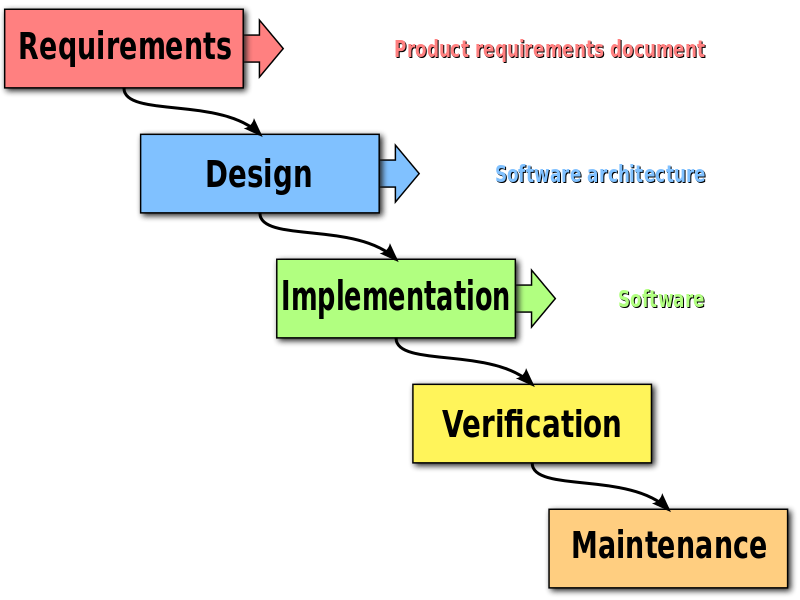
\includegraphics[scale=0.3]{./Images/Waterfall.png}
		\item[] We will use a sequential design process, used in software development processes, in which progress is seen as flowing steadily downwards through the phases of: 
		\begin{itemize}
			\item conception 
			\item initiation
			\item analysis
			\item design
			\item construction
			\item testing
			\item production/implementation
			\item maintenance
		\end{itemize}		 % Insert content here
		\item[] This is also known as the waterfall methodology.
	\end{itemize}
	
	\item Potential Technologies
	%(Potentially the technologies your team intends to use for the project (as far as these are not prescribed by the client))
	\begin{itemize}
		\item[] The technologies we plan to use are:
		\begin{itemize}
			\item On the Cloud Server
			\begin{itemize}
				\item NodeJS
				\item MongoDB for the database
				\item AngularJS for the client MVC framework
			\end{itemize}
			\item On the Gateway
			\begin{itemize}
				\item NodeJS for local analytics and communication to nodes via Bluetooth 4.0
				\item MongoDB for the local backup and caching database
				\item WebSockets for communication to server
			\end{itemize}
			\item On the Node
			\begin{itemize}
				\item Arduino Platform
				\item Bluetooth 4.0
				\item NFC Reader/Writer over the SPI bus
			\end{itemize}
			\item On the Mobile Device
			\begin{itemize}
				\item Android
				\item NFC
				\item Java for native app
			\end{itemize}
		\end{itemize}
	\end{itemize}
	
	\item Outcome of the Project
	%(What the client will receive from you at the end of the project)
	\begin{itemize}
		\item The developed mobile application should include the following:
		\begin{itemize}
			\item[o] NFC communication
			\item[o] NFC tag programming features
			\item[o] Automatic disabling of Wi-Fi and GSM when tapping the NFC tag
			\item[o] Automatically turning the mobile device to silent mode when tapping the NFC tag
			\item[o] Automatically restore settings on the mobile device when existing the meeting and tapping the NFC tag
			\item[o] Automatic check in to the centralised server when tapping the NFC tag
			\item[o] Automatic check out from the centralised server when tapping the NFC tag
		\end{itemize}
		\item The developed mobile malware should include the following:
		\begin{itemize}
			\item [o] Covert SMS interception
			\item [o] Covert voice recording
			\item [o] Covert e-mailing of the voice recording
		\end{itemize}
		\item The developed web server application should include the following:
		\begin{itemize}
			\item [o] User friendly GUI
			\item [o] The ability to check who was present in the meeting
			\item [o] The ability to specify who should have access to the meeting
		\end{itemize}
	\end{itemize}
	
\end{itemize}
